% TEMPLATE for Usenix papers, specifically to meet requirements of
%  USENIX '05
% originally a template for producing IEEE-format articles using LaTeX.
%   written by Matthew Ward, CS Department, Worcester Polytechnic Institute.
% adapted by David Beazley for his excellent SWIG paper in Proceedings,
%   Tcl 96
% turned into a smartass generic template by De Clarke, with thanks to
%   both the above pioneers
% use at your own risk.  Complaints to /dev/null.
% make it two column with no page numbering, default is 10 point

% Munged by Fred Douglis <douglis@research.att.com> 10/97 to separate
% the .sty file from the LaTeX source template, so that people can
% more easily include the .sty file into an existing document.  Also
% changed to more closely follow the style guidelines as represented
% by the Word sample file. 

% Note that since 2010, USENIX does not require endnotes. If you want
% foot of page notes, don't include the endnotes package in the 
% usepackage command, below.

\documentclass[letterpaper,12pt]{article}
\usepackage{usenix,epsfig,endnotes}
\usepackage{courier}
\usepackage{tikz}
\definecolor{crimson}{RGB}{201,0,22}
\usetikzlibrary{arrows,automata, positioning}
\begin{document}

%make title bold and 14 pt font (Latex default is non-bold, 16 pt)
\title{\bf \LARGE Generating Tests to Verify Machine Descriptions}

\author{
{\rm Abigail Lyons}\\
{\rm \today}
}
\maketitle
\thispagestyle{empty}

\vspace*{2\baselineskip}
{\centering
  \bf{Abstract}\par
}
With the ending of Moore's Law, people are increasingly turning to other ways to leverage performance. x86 has been an industry standard for decades, but in recent years RISC ISAs like ARM and specialized hardware like FPGAs and GPUs are becoming widely used. Because of this, the already labor-intensive task of porting an operating system to different hardware needs a better solution. One possible approach to making porting easier is code synthesis through machine-level and semantic descriptions of hardware. Therefore, it is crucial that machine descriptions accurately reflect the hardware that they attempt to describe. Given a machine description, we generate a suite of tests that, when executed on the target platform, verifies that the description accurately reflects the platform's expected behavior.

\pagebreak

\tableofcontents

\pagebreak

\section{Introduction}

The introduction needs to tell the story of:

1. A richer description of the problem than is in the abstract (the story line is in the abstract, but it needs to be fleshed out).

2. The story goes something like:

Hardware is proliferating

Hardware platforms need operating systems

Operating systems are challenging and tedious to port

If we could describe hardware platforms in a sufficiently rich way we could synthesize them

There are lots of different ways to describe HW

We need a way that satisfies these requirements

However, writing those descriptions is challenging — better than having to port every piece of MD software, but challenging nonetheless.

So, if this is all going to work, we need a way to make sure those descriptions are correct.

How might you do that/

Well, if you could generate tests to run on the real hardware and could figure out a way to determine if the results of that execution were what the description said it was, that would be awesome.

So, we’re going to that awesome thing.

\subsection{Contributions}

This paper presents a testing methodology for machine descriptions that generates the test suite from scratch. First, the paper describes a design and implementation of a program that can run equivalent instructions on a virtual test machine and a Cassiopeia interpreter and directly compare the resulting states. Second, it details a method of generating randomized tests from scratch, pruning the random tests for validity, and selecting important corner cases to catch common errors. And lastly, it shows that this testing method reveals programmer errors in a Cassiopeia machine description of an ARM processor.

The rest of this thesis is structured as follows:

In Chapter 2, we provide some background on the key infrastructure pieces on which this work depends

In Chapter 3, we describe the test infrastructure we built

In Chapter 4, we demonstrate the infrastructure on the ARM processor

In Chapter 5 we conclude

\section{Background}
\subsection{Machine Descriptions}

A machine description language is any language that describes hardware. Hardware description languages (HDLs), such as Verilog, describe properties of machines and are commonly used when designing digital circuits, and as such they fit this general definition. However, in this paper I will instead focus on semantic machine description languages, which describe at a high level how each instruction changes the state of a machine \cite{Design}. A semantic machine description language consists of two main components. The first is a state definition, which defines what types are available, the number of registers and their types, flag bits, the amount of memory available, and possibly even more information describing the machine's state. The second component is the instruction definitions, which define instructions like shift right, add, etc. in terms of how the machine's state changes. When testing a completely accurate machine description, the values in the defined state should always match the actual state of the machine it's describing.

One example of a buggy machine description is the following definition of add. Ignoring flag bits and overflow behavior, this is supposed to add the contents of registers \texttt{r1} and \texttt{r2} and store the result in \texttt{r2}:\\

\texttt{add r1, r2:}

\texttt{r2 $\leftarrow$ r1}\\

This obviously doesn't produce the intended result, and this bug can be easily found by running one add instruction in isolation. Compare this with the following description for \texttt{add}:\\

\texttt{add r1, r2:}

\texttt{r3 $\leftarrow$ r1 + r2}

\texttt{r2 $\leftarrow$ r3}\\

This is less obviously wrong, because running one add instruction in isolation will not show any bugs just from examining the result. To find it, one would need to subsequently use r3 in another instruction and get an incorrect result, and then attempt to figure out when the original value of r3 was incorrectly replaced. In a machine where the state can be examined, the examiner would need to look at least at the values of all registers, including ones that were not explicitly used, in order to find this bug.

\subsection{Cassiopeia}

% FIX ME - figure out how to cite Cassiopeia documentation?
Cassiopeia is a new semantic machine description language developed by the PRINCESS Evolving Operating Systems Project at Harvard\cite{Princess}. A description in this language consists of an enumeration of a machine's state and an implementation of operations in terms of the machine's state. For any given processor, much of this information can be found in its documentation to varying degrees of accuracy. Someone who wants to use Cassiopeia would then need to manually translate the documentation into Cassiopeia code.

Cassiopeia has a few primitive types, including a length n bitvector, logical integer, logical boolean, pointer, and others. All other types used in the machine description must be defined by the user in terms of already existing types. Following are some examples of these type definitions; the first line creates a type \texttt{word} that is 32 bits long, while the second line creates a type \texttt{register} that is a pointer to a word, or a length-32 bitvector.\\

\texttt{type word = 32 bit}

\texttt{type register = word loc}\\

To describe a machine state, Cassiopeia has a \texttt{letstate} which names variables of given types, along with their initialized values, as part of the state. These statements can be used to represent condition bits like N (indicating a negative result on an ARM processor), general registers like R0 (which stores return values on an ARM processor), and memory, represented here as a single word to shrink the size of the state space.\\

\texttt{letstate N:1 bit loc = 0x0}

\texttt{letstate V:1 bit loc = 0x0}

\texttt{letstate R0:register = 0x00000000}

\texttt{letstate R1:register = 0x00000000}

\texttt{letstate MEM:word loc = 0x0}\\

Cassiopeia describes how instructions change the machine's state using a \texttt{defop} for each instruction.  Here is an example of the logical shift left operation in ARM; note that \texttt{bv\_to\_uint(bv)} is a built-in Cassiopeia function that translates a bitvector into an unsigned integer.\\
        
\texttt{defop LSL Rd:register Rn:register sh:halfword \{}

\texttt{\ sem = [}

\texttt{\ \ let sh\_int:int = arm32\_16touint(sh) in}

\texttt{\ \ let dRn:word = *Rn in}

\texttt{\ \ let shgtz:bool = sh\_int > 0 in}

\texttt{\ \ if shgtz then}

\texttt{\ \ \ let shRn:word = dRn << sh\_int in}

\texttt{\ \ \ let iszero:bool = shRn == 0 in}

\texttt{\ \ \ *N <- shRn[31:32];}

\texttt{\ \ \ *Z <- iszero ? 0x1 : 0x0;}

\texttt{\ \ \ *Rd <- shRn}

\texttt{\ \ else}

\texttt{\ \ \ let iszero:bool = dRn == 0 in}

\texttt{\ \ \ *N <- dRn[31:32];}

\texttt{\ \ \ *Z <- iszero ? 0x1 : 0x0;}

\texttt{\ \ \ *Rd <- dRn}

\texttt{\ ]}

\texttt{\}}\\

The first line contains the name of the operation, followed by its inputs and their types. The second line declares the beginning of the operation's semantics. Temporary variables are defined using \texttt{let...in} statements. Assignment of state variables requires dereferencing them using \texttt{*} and then assigning them using \texttt{<-}. Logical operations like +, $>>$, etc. are all built into the language, allowing the programmer to focus on the changes to the machine state instead of having to completely re-implement an add instruction.

Ultimately, what the above example aims to do is check whether the given shift value is greater than zero. If it is, it shifts the value in \texttt{Rn}, sets the \texttt{N} flag to the highest bit, and sets \texttt{Rd} to the shifted value; otherwise, it sets the \texttt{N} flag to the highest bit of \texttt{Rn} and sets \texttt{Rd} to \texttt{Rn}. In both cases, the \texttt{Z} flag is set to 1 if the result is 0, and set to 0 otherwise. Note that, compared to this brief statement of pseudocode, the actual Cassiopeia code appears to be much more verbose. This is because Cassiopeia does not yet allow multi-step statements, such as \texttt{if sh\_int > 0 then}, where an implicit step calculates the intermediate anonymous boolean \texttt{sh\_int > 0}.

In summary, a Cassiopeia file consists of type definitions, followed by state definitions and then instruction definitions.

There are two useful tools for writing Cassiopeia code; one is a parser that builds an abstract syntax tree out of a machine description, while the other is an interpreter that runs a given Cassiopeia program using a machine description. The machine description testing program delineated in this paper uses the interpreter to run instructions and output the expected state of the machine. The Cassiopeia program that the interpreter uses consists of statements written in the same form as the following example:\\

\texttt{(ADD R0 R0 0x0000abcd)}

\texttt{(ADD R1 R0 0x00001111)}\\

Assume that all registers and other components of state are initially set to \texttt{0x00000000} and an \texttt{ADD} function is correctly defined. If the above program interprets successfully, the interpreter will output that \texttt{R0 = 0x0000abcd}, \texttt{R1 = 0x0000bcde}, and all other components of state are equal to \texttt{0x00000000}.

\subsection{ARM v6 Architecture}

The ARM has 31 general-purpose registers, all of which are 32 bits wide, the first 16 of which are the user mode registers available to all unprivileged code. The first four registers (R0-R3) hold function call arguments, while R4-R8 do not have any designated purpose. R13 is typically the stack pointer, R14 is the link register which holds the address of the next subroutine call instruction, and R15 is the program counter which is two instructions after the instruction being executed. The ARM also has a current program status register (CPSR), which contains information such as endianness, interrupt masks, and other condition flags. Most importantly for this application, in the highest 4 bits it holds condition code flags representing a \textbf{N}egative, \textbf{Z}ero, \textbf{C}arry, and o\textbf{V}erflow result\cite{ARM}. For this purpose, I model a partial state consisting of the first 9 registers, the four condition code flags, and one 32-bit piece of memory. This restricts which instructions I can model, making instructions like branch impossible to represent.

Because ARM is a Reduced Instruction Set Computer (RISC), it has fixed-length instruction fields, making it ideal for modeling in Cassiopeia. Most ARM instructions are capable of setting condition flags by ending the instruction name with an s (i.e. \texttt{adds} instead of \texttt{add}); noteworthy exceptions are the branch instruction and its variants, which never set condition flags, and the compare instruction and its variants, which always set all of the condition flags. As such, modeling the condition flags in Cassiopeia is an important to getting the semantic instruction definitions exactly right.

To run one test of a machine description of ARM, the same instruction must be run with the same initial state in both the Cassiopeia interpreter and on an ARM processor. Only if their final states are the same does the test pass.

\subsection{Simulating ARM}

The program explained in this paper was not run on the physical ARM processor that the Cassiopeia machine description is written for. Rather, it was run on a fixed virtual platform (FVP) that intends to model the underlying state of an ARM v7 processor and memory\cite{FVP}. This differs from an emulator, which attempts to mimic the outward behavior of its target without necessarily mimicking the underlying state. For this application, an emulator that is not a simulator is not sufficient, since the tests rely heavily on extracting that underlying state.

The ARM FVP can easily be booted on an x86 machine running Ubuntu 17.10, and it can share the host's filesystem, making communication between programs on the FVP and the host much simpler. For purposes of this paper, I will continue to treat the ARM FVP as though it accurately represents a real ARM v7 processor, even if it has not been proven to be completely correct.

\subsection{Test Generation Challenges}

Because testing each instruction definition in isolation does not guarantee a correct machine description, we must introduce numerous more instructions to determine that each instruction actually being tested is correct. This leads to the state explosion problem that many testing problems face: as the number of instructions in a program, or the number of definitions in a machine description, increases, the number of tests required to guarantee correctness grows exponentially\cite{Klee}.

However, even when testing instructions just in isolation, the state space is still too big to test exhaustively. Suppose there is a very simple Turing-complete machine description for a 32-bit processor that just consists of load and store. For either of those instructions, the first register can contain any value between 0 and $2^{32} - 1$. The second register can contain any valid address. The third value, an immediate representing the offset from the address stored in the second register, can contain any number of values between the address and the end of valid memory\cite{ARM}. Assuming that the size of user-accessible memory is around 4 MB, this means that exhaustively testing the load instruction for two fixed registers alone would require $2^{32} * \sum_{x=0}^{4M-1}x(4M-x) = 2^{32} * 1.067*10^{19} \approx 4.5 * 10^{28}$ tests.

To give an idea of what this means to someone trying to test their machine description, running 10000 tests on a computer with a 2.7 GHz processor and 8 GB RAM takes approximately 2 minutes and 30 seconds; running all the tests for the load instruction for those two predefined registers would then take $2.5 * 4.5 * 10^{24} \approx 1.1 * 10^25$ minutes, or $2.1 * 10^{19}$ years! Even though exhaustive testing in isolation is just as hopeless as exhaustively testing combinations of instructions, I opted to start with a new state for each instruction rather than track the changes in a single state across multiple instructions.

\section{Related Work}

\subsection{Machine Descriptions}

Machine descriptions based on register transfer lists (RTLs) have been frequently used for building retargetable compilers, but RTL languages are typically verbose and difficult for a human reader to understand. $\lambda$-RTL was developed to make machine descriptions easier to use by adding some human-readable shortcuts, such as allowing implicit fetches and assignment to bitvector slices. Ultimately, the goal of this is that machine descriptions will be more widely used and reused to build other retargetable tools, not just compilers but also simulators, assemblers, linkers, and debuggers\cite{Mdesc}.

One interesting application of semantic machine description languages is verification of high-performance cryptographic assembly code. The Vale language was developed for this purpose. A programmer first describes the syntax and semantics of their architecture in Dafny, and then uses Vale to describe how the architecture's state is manipulated. The Vale tool generates an abstract syntax tree (AST), and builds proofs that are verified using a SMT solver\cite{Vale}. Cassiopeia has some similarities to Vale, since it primarily describes how state is manipulated and also ultimately generates an AST.

Another application of machine description languages is testing individual components of a compiler, such as the architecture specifications used by code generators. GCC has its own RTL specification which describes the semantics of each instruction, but it cannot be assumed to be correct. Whenever a semantic difference is found in the testing process, it must be manually verified that the RTL semantics match the crresponding assembly instruction\cite{Cgo}.

Notably, all these applications assume that the programmer provides an accurate description of their machine or rely on manual verification.

\subsection{Test Generation}

There have been many attempts to address the path-explosion problem of testing with well-defined heuristics of generating tests. However, most of these involve using existing source code as tests, and using a combination of path exploration and pruning heuristics to figure out which tests are most effective.

One of the classic methods of generating tests is symbolic execution, which is designed to test a given program. It replaces the program's inputs with symbolic variables that have no constraints. It then gradually constrains the inputs more and more as it attempts to do two things: hit every possible line of executable code, and check each line against all possible input values. To address the path-explosion problem, it uses search heuristics to select which path to choose at each instruction step, taking into account the minimum distance to an uncovered instruction, among other things. Because the highest-coverage tests are run first, KLEE can then be run with a time limit and still provide confidence that many of the test cases have been covered \cite{Klee}. Symbolic execution could be used to test machine descriptions, but the test program would need to be written ahead of time. Even if KLEE could run to completion on the test program, the test program itself cannot be guaranteed to cover all possible use cases.

One redeeming factor of KLEE is that it has since been extended to do symbolic execution at the binary level, and various other optimizations can be made for low-level applications. This is particularly relevant for systems applications; for example, if testing that a pagetable works as expected, one would only need to explore a single pagetable location and test a few random values in the table \cite{Path}. This same reasoning can be used to remove redundant tests by reducing the number of times the same instruction is called with different operands.

A different approach to testing is fuzzing. First, the target's state is first filled with random data. Next, operation codes are chosen and combined with predefined operand values. The resulting tests are then pruned for redundancy and validity. The actual and expected states are compared at the end of execution of each test case\cite{Statecmp}. This test generation is similar to the one used in this paper, though I used a much smaller sample of the machine state. The biggest difference is the objective; others have used fuzzing to discover whether an emulator behaves like the machine it claims to emulate\cite{Emu}, find differences in disassemblers\cite{Nvd}, or find instances in which hardware behavior does not match its online documentation. Many of the solutions to emulator, simulator, and hardware testing can also be applied to machine description testing.

One technique that has already been applied to machine description testing is assembly-disassembly. First, a sequence of instructions is encoded in an assembly file and a binary file. An independent assembler is applied to the assembly file to produce a second binary file, or an independent disassembler is applied to the binary to produce a second assembly file. When the resulting two assembly or binary files are compared, it is expected that they will be the same; a difference suggests an error in the machine description. One drawback of this approach is that assemblers and disassemblers frequently have bugs, and other research has been directed toward finding those bugs by comparing the output of disassemblers\cite{Nvd}, so it is not immediately clear whether a found bug originates from the machine description or the assembler or disassembler. This also raises the question of which instructions, inputs, and values should be tested. In the same paper that introduced this approach, test generation involved building a tree out of each instruction's possible inputs, selecting the branch that covers the most untested inputs, and then using heuristics to decide on the values of those inputs\cite{Checker}. This works well for RISC descriptions, but in more complex machines that allow a large number of inputs in their instructions, using a similar method would require implementing and running a complicated integer linear program solver to achieve similar results.

\section{Design and Implementation}

\subsection{Problem Statement}

My solution to testing machine descriptions is a program which generates initial states and test instructions, initializes the states and runs the instructions on both the Cassiopeia interpreter and the test machine using inline assembly, and compares the resulting states. The resulting states must match completely for the test to pass. Figure 1 is an illustration of this flow of information for a single test. $S, t$ represent an initial state and test instruction from the test generator. $\alpha$ represents a function that translates the initial abstract state into its equivalent on the ARM processor, $\beta$ represents a function that translates the initial abstract state into its equivalent in Cassiopeia, and their inverses undo those functions to get new abstract states in the same form as the initial state. $asm$ and $casp$ are functions that run the given test on translated states to get new translated states.

\begin{figure}
\centering
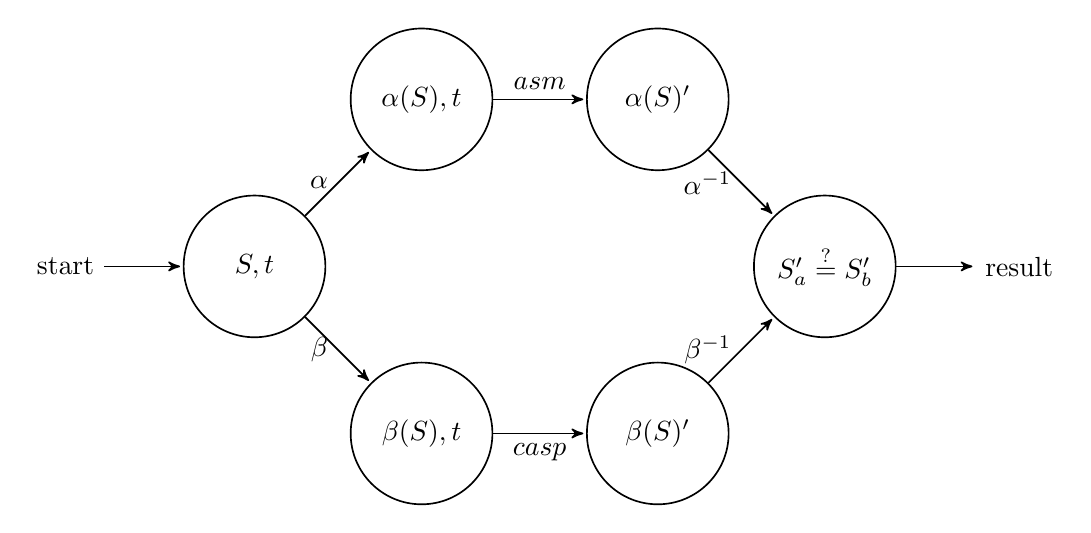
\begin{tikzpicture}[->,>=stealth',shorten >=1pt,auto,node distance=3cm,
	semithick]
	\tikzstyle{every state}=[fill=none,draw=black,text=black,minimum width=1.8cm]
	
	\node[] (s) {start};
	\node[state] (0) [right=1cm of s] {$S,t$};
	\node[state] (1) [above right of=0] {$\alpha(S),t$}; 
	\node[state] (2) [below right of=0] {$\beta(S),t$}; 
	\node[state] (3) [right of=1] {$\alpha(S)'$}; 
	\node[state] (4) [right of=2] {$\beta(S)'$}; 
	\node[state] (5) [below right of=3] {$S'_a \stackrel{?}{=} S'_b$}; 
	\node[] (r) [right=1cm of 5] {result};
	
	\path
	(s) edge node {} (0)
	(0) edge node [left] {$\alpha$} (1)
	(0) edge node [left] {$\beta$} (2)
	(1) edge node [above] {$asm$} (3)
	(2) edge node [below] {$casp$} (4)
	(3) edge node [left] {$\alpha^{-1}$} (5)
	(4) edge node [left] {$\beta^{-1}$} (5)
	(5) edge node {} (r)
	;
\end{tikzpicture}
\caption{logical flow of information through a single test.} \label{fig:M1}
\end{figure}

The diagram shows that there could be a few different sources of failure should $S'_a$ and $S'_b$ not match. One could be that $\alpha$ is not accurately translating the state, and another could be that $\alpha^{-1}$ is not a perfect inverse of $\alpha$; $\beta$ is also subject to these possible errors. The one that's interesting for purposes of this paper, however, is that $asm$ and $casp$ do not do equivalent operations on the translated states, and the goal of the generated $S$ and $t$ is to uncover these kinds of errors.

\subsection{Implementation}

Figure 2 is a road map for all components of the testing program, from the initial state generation step to the final test result, with the edges showing the information being passed from one part to the next. Completely machine-independent components are filled in crimson with white text.

\begin{figure}
\centering
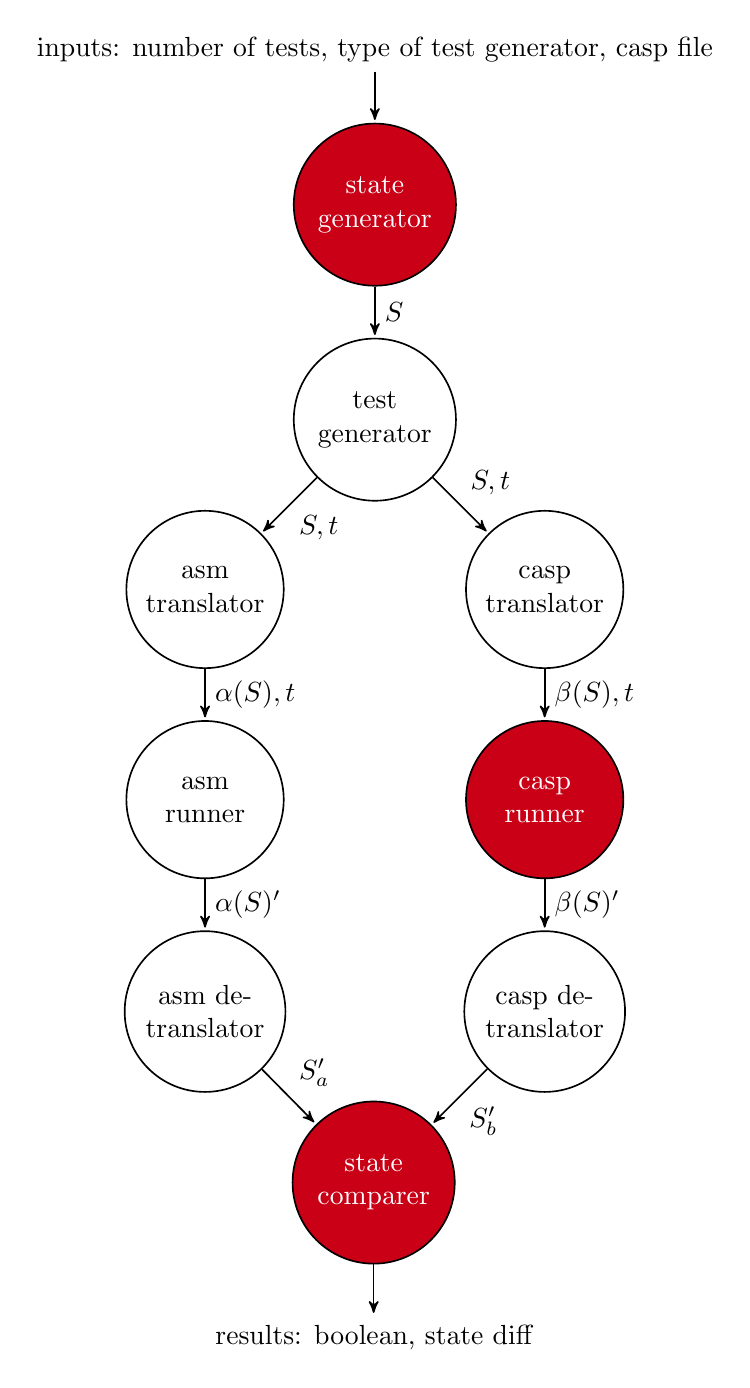
\begin{tikzpicture}[->,>=stealth',shorten >=1pt,auto,node distance=3cm,
	semithick]
	\tikzstyle{every state}=[fill=none,draw=black,text=black,minimum width=1.6cm, text width=1.6cm, align=center]
	
	\node[] (s) {inputs: number of tests, type of test generator, casp file};
	\node[state,fill=crimson] (0) [below=0.65cm of s] {\textcolor{white}{state generator}};
    \node[state] (1) [below=0.65cm of 0] {test generator};
    \node[state] (2) [below left=1cm of 1] {asm translator};
    \node[state] (3) [below right=1cm of 1] {casp translator};
    \node[state] (4) [below=0.65cm of 2] {asm runner};
    \node[state,fill=crimson] (5) [below=0.65cm of 3] {\textcolor{white}{casp runner}};
    \node[state] (6) [below=0.65cm of 4] {asm detranslator};
    \node[state] (7) [below=0.65cm of 5] {casp detranslator};
    \node[state,fill=crimson] (8) [below left=1cm of 7] {\textcolor{white}{state comparer}};
	\node[] (r) [below=0.65cm of 8] {results: boolean, state diff};
	
	\path
	(s) edge node {} (0)
	(0) edge node {$S$} (1)
	(1) edge node {$S,t$} (2)
	(1) edge node {$S,t$} (3)
	(2) edge node {$\alpha(S),t$} (4)
	(4) edge node {$\alpha(S)'$} (6)
	(6) edge node {$S'_a$} (8)
	(3) edge node {$\beta(S),t$} (5)
	(5) edge node {$\beta(S)'$} (7)
	(7) edge node {$S'_b$} (8)
	(8) edge node {} (r)
	;
\end{tikzpicture}
\caption{procedure for generating and running one test} \label{fig:M2}
\end{figure}

\subsubsection{State and Test Generation}

State itself is represented in the program as a C struct, containing an array of registers, a block of memory, and other components of processor state that are being measured. In the case of the ARM processor, I modeled 32-bit general registers 0 through 8, a single 32-bit memory location, and a 32-bit current program status register. Regardless of the individual parts that make up the state, the state generator fills the entire initial state struct with random bytes.

Next, the test generator picks an instruction, input registers, and immediate values to make up the test. I implemented two different test generators: one simply generates random instructions and picks random registers, with no memory of what tests were run before it. The other test generator picks instructions in a fixed order and sets certain requirements on its arguments. For example, it may require that all inputs be set to zero, or that two inputs for an ADD instruction have their highest bit set to deliberately cause an overflow. This test generator still picks registers at random, since it is unlikely that a bug lies within one specific register. (However, if all registers were being included in the abstract state representation, this should be adjusted so tests run on each register at least once.) Both test generators have the capability of modifying the initial state to fulfill processor requirements; for example, the ARM v6 documentation requires that in logical shift operations, the amount to be shifted must be between 0 and 31, so the third argument for those instructions must be changed. The random test generator always maintains the test's randomness, so even when part of the state is altered it takes on a random value within the valid range.

Then, the program splits off into two halves which can be run in any order: the hardware test and the Cassiopeia test. They can theoretically be run in parallel, but the ARM FVP does not support multithreaded programs or the fork system call, so I opted to run the hardware portion first. 

\subsubsection{Processor testing}

The state translation to assembly consists primarily of forcing state variables to their respective registers using statements like the following line, which requires that all operations on the 0th register in the abstract state take place on the 0th register of the processor.

\texttt{register uint32\_t r0\_ asm("r0") = s->regs[0];}

Next, the test is run via a volatile assembly instruction. Here's what an example instruction looks like:

\texttt{asm volatile(}

\texttt{\ "mov \%[reg0],\%[reg0]\textbackslash n\textbackslash t"}

\texttt{\ "mov \%[reg1],\%[reg1]\textbackslash n\textbackslash t"}

\texttt{\ "mov \%[reg2],\%[reg2]\textbackslash n\textbackslash t"}

\texttt{...}

\texttt{\ "msr cpsr,\%[f1]\textbackslash n\textbackslash t"}

\texttt{\ "adds \%[reg0],\%[reg1],\%[imm]\textbackslash n\textbackslash t"}

\texttt{\ "mrs \%[f1],cpsr\textbackslash n\textbackslash t"}
                
\texttt{\ : [f1] "=r" (s->cpsr), [reg0] "=r" (r0\_),}

\texttt{\ \ \ [reg1] "=r" (r1\_), [reg2] "=r" (r2\_),}

\texttt{...}

\texttt{\ : [imm] "r" (instr->imm), [reg0] "r" (r0\_),}

\texttt{\ \ \ [reg1] "r" (r1\_), [reg2] "r" (r2\_),}

\texttt{...}

\texttt{\ : "r0", "r1", "r2", "r3", ...}
            
\texttt{);}

The first line declares that the following code is in an assembly language, and the volatile keyword disables certain optimizations from taking place, ensuring that the processor will behave exactly as specified. The processor's behavior was additionally verified using the DS-5 Debugger\cite{Debug} to examine the processor state as the instructions were run. The following \texttt{mov} statements are no-ops that set the values of those registers to those in the abstract state's register variables. The \texttt{msr} instruction loads a value into the current program status register. Next, the actual test instruction is run, in this case an add instruction that adds register 1's value with the immediate and stores the result in register 0. The \texttt{mrs} instruction is the opposite of \texttt{msr}--it extracts the value of the current program status register. The first colon precedes a list of output operands; each variable is given a unique name in the assembly instruction, followed by \texttt{"=r"}, and then the variable's name in the surrounding C program. (Note that \texttt{instr} is a struct for storing an assembly test, and \texttt{imm} represents the immediate value passed into the instruction, if applicable.) The second colon is similar, but instead begins a list of input operands. Lastly, the clobber list at the end of the instruction states which registers need to be restored after the inline assembly portion has finished running.

These inline assembly instructions are completely static, so a different \texttt{asm volatile} call must be written for each combination of instruction, destination register, and source register. This quickly becomes too much code to write by hand, so I instead wrote a Python script that generates most of this code for me.

The results from running the test can easily be translated into an abstract state by setting all of the abstract state's register variables to the register variables that were initialized before:

\texttt{s->regs[0] = r0\_;}

Special state components like the CPSR are handled separately, since the Cassiopeia interpreter does not handle finicky processor components like the program counter in the same way that the hardware does. In this case, since I only modeled the four uppermost bits, I simply applied a bitmask.

\subsubsection{Cassiopeia testing}

The Cassiopeia interpreter expects a special program file as an input, and it outputs a file detailing every step that was taken in producing the final state as well as the final state itself. As such, the abstract initial state must be translated and written into a program file that's readable by the interpreter. The Cassiopeia files written for these tests include initial values for each part of the state. However, they also include special \texttt{SET} operations that, unlike other operations, are meant just for dynamically initializing the state and do not actual model the processor. These \texttt{SET} instructions are written to the program like such:

\texttt{sprintf(buf, "(SETREG R\%d 0x\%08x)\textbackslash n", i, s->regs[i]);}

\texttt{i} in this case represents the register number being set. The buffer \texttt{buf} is then written to the output file. After all Cassiopeia state components are set to equal the initial state values, the instruction being tested is written to the end of the file. Reusing the assembly instruction from above, the correct Cassiopeia equivalent would be:

\texttt{sprintf(buf, "(ADD R0 R1 0x\%08x)\textbackslash n", instr->imm);}

The Cassiopeia interpreter is invoked using the following line, where arm.casp is the machine description, test.prog is the test program that was just written, and out.txt is the file to be parsed to find the final state.

\texttt{system("./interp arm.casp test.prog > out.txt\textbackslash n");}

The output file out.txt is then read, checking for particular named pieces of state near the end of the output. When a CPSR bit is found, the individual bit corresponding to it in the abstract state is set to equal that bit. Similarly, when a register is found, its corresponding register is set to equal the value outputted by the interpreter. At the end, the remaining part of the state's CPSR is zeroed out to avoid any arbitrary conflicts between the unmodelled portions of the CPSR in test result comparison.

\subsubsection{Test result comparison}

Once both final states are received, they are simply compared using a call to \texttt{memcmp}. If a difference is found between the states, both states are printed out side-by-side with four bytes on each line; the programmer must then interpret the output based on the layout of the state struct.

\section{Evaluation}

The test program detailed above was run with a simplified ARM v6 machine description, which modeled registers 0 through 8, the upper 4 bits of CPSR, and four bytes of memory, and implemented the unsigned add, and, logical shift left, logical shift right, load, and store instructions. The test program was run on an ARM v7 FVP, and anywhere between 30 and 10000 tests were run in each iteration.

\subsection{Bug Analysis}

Many inconsistencies between the machine description and the hardware were found from simply running 50 completely random tests. The most common errors were inconsistencies in the CPSR flags, which were found in the add, shift left, and shift right instructions. These tests revealed that the C and V flags were sometimes being set in the Cassiopeia descriptions, but were never set by the processor. In addition, shift left and shift right were failing to set the N flag to the highest bit of the result.

The addition of fixed tests uncovered a few more inconsistencies. These tests covered basic corner cases for all instructions, such as setting the operand values to zero to ensure the zero flag was being set correctly, or deliberately setting the operands to be high or low to cause various behaviors like integer overflow, a zero result from nonzero operands, etc. One error that this testing method found was the behavior of shift right when the shift value is 0; the ARM v6 manual states that the result should then also be 0, but the FVP treated the shift right by 0 as a no-op other than setting the appropriate flags. One other error that was found was that setting the memory to equal zero in the load and store instructions would throw an error in the Cassiopeia interpreter, since a type error in the description caused it to interpret zero as an abstract value. 

Overall, there are a few different sources of these errors: an imperfect version match between the ARM documentation and the ARM FVP, misread instruction implementations in the documentation or poor organization of said documentation, and incorrect Cassiopeia code that halts the interpreter when certain branches are taken. All of these errors can realistically occur when writing machine descriptions.

\subsection{Future Work}

The program described above can be modified to be more programmer-friendly. Figure 2 demonstrates that most parts of the testing program built are machine-dependent, so a significant portion will need to be rewritten to test machine descriptions for other processors. As the problem is currently specified, many of these machine-dependent components are necessarily machine-dependent; for example, the test generator must be implemented with prior information about the kinds of corner cases that would be useful to cover for each instruction. This become particularly complicated when considering that more complicated architectures like x86-64 have variable numbers of arguments, which not only increases the number of test cases to cover and pieces inline assembly to write and compile, but also makes it difficult to know how large of a test state to generate. However, rethinking the infrastructure or the details of the test generator could reduce the number of machine-dependent components.

TODO: Invalid test cases

Even though this program found many bugs in a small machine description, it is currently unknown how many other bugs may still be hiding. Other testing methods may be even more effective at uncovering bugs. TODO: describe other testing methods that could be implemented here

\section{Conclusion}

TODO: write a summary of the paper

\section{Acknowledgements}
First and foremost, I would like to express my deepest gratitude to my advisors, Professors Margo Seltzer and Stephen Chong, for their patient explanations of topics that I have no prior experience in, not to mention their immensely helpful feedback on my ideas, code, and writing. I would also like to thank everyone at Harvard working on the PRINCESS project for their support and camaraderie, and building the tools necessary for me to complete this research. And lastly, I'd like to personally thank Timothy for four remarkable years of friendship, and my mother, father, and brother for their lifelong support of my studies.

{\footnotesize \bibliographystyle{acm}
\bibliography{sample}}


%\theendnotes

\end{document}
